\begin{Exercise}[title=($*$) Télémètre]
Un télémètre est un appareil permettant de mesurer une distance à l’aide d’une approche optique.
%\begin{figure}[h]
	\begin{center}
		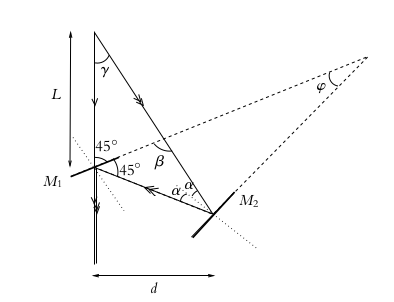
\includegraphics[scale=0.5]{./fig/telemetre.png}
	\end{center}
%\end{figure}

On considère un dispositif constitué de deux miroirs, l’un totalement réfléchissant et l’autre semi-réfléchissant.
Le premier $M_2$ est un miroir classique tandis que le second $M_1$ permet au rayon d’être réfracté lorsqu’il arrive sur la surface non réfléchissante.
Les deux miroirs sont inclinés d’un angle $\phi$ l’un par rapport à l’autre.
On place une source ponctuelle S du côté de la face non réfléchissante du miroir $M_1$ à une distance L du centre $O_1$ de $M_1$. Un rayon incident arrive sur $M_1$ en $O_1$ avec une incidence de 45\si{\degree}et traverse $M_1$.
Un autre rayon arrive sur $M_2$ avec une incidence a au centre $O_2$ de $M_2$ , il est réfléchi sur $M_2$ puis sur la surface réfléchissante de $M_1$ . On tourne $M_2$ jusqu’à superposer les deux images. On note d la distance de $O_2$ aux rayons émergeant du système.
\Question En assimilant $M_1$ à une lame à faces parallèles lorsqu’il est traversé par les rayons, montrer
qu’alors le rayon émergent est parallèle au rayon incident.
\Question On note $\beta$ l’angle entre la direction du rayon $SO_2$ et celle du miroir semi-réfléchissant $M_1$ .
Établir la relation entre $\beta$ et $\phi$.
\Question En déduire la relation entre $\phi$ et $\gamma$ l’angle entre $SO_1$ et $SO 2$ .
\Question Montrer que ce dispositif permet de déterminer $L$ si on connaît $d$ et la valeur de $\phi$ pour que les deux images se superposent.
\end{Exercise}
\begin{Answer}
\Question L’application des relations de Descartes donne $\sin i = n \sin r = \sin i'$ soit $i = i'$ : les rayons incident et émergent sont parallèles.
\Question La somme des angles d’un triangle est égale à $\pi$ soit en appliquant cette relation aux triangles $O_1 AO_2$ d’une part $\frac{\pi}{4}+\beta+2\alpha = \pi$ et d’autre part $AO_1B$  $\pi-\beta +\frac{\pi}{2}-\alpha+\phi=\pi$ Alors en éliminant $\alpha$ entre les deux relations, on en déduit $\beta = \frac{\pi}{4} +2\phi$.
\Question La somme des angles d’un triangle est égale à $\pi$ soit pour $SO_1A$ : $\frac{\pi}{4}+\gamma+\pi-\beta = \pi$ En tenant compte du résultat de la question précédente, on en déduit $\gamma =2\phi$
\Question L’expression de la tangente dans le triangle rectangle donne $\tan 2\phi = \frac{d}{L}$ont on déduit $L=\frac{d}{tan 2\phi}$.
\end{Answer}
